%!TEX root = ../main.tex

% chktex-file 1
% chktex-file 44
% chktex-file 13

\documentclass[../main]{subfiles}

\begin{document}

\subsection{OpenQCD}\label{sec:openqcd}

OpenQCD-FASTSUM\footnote{\url{https://gitlab.com/fastsum/openqcd-fastsum/}} is a code for Lattice QCD simulations.
The main development is in C, with some functions heavily optimized using intrinsics from various instruction sets.
This work builds upon previous DiRAC work, where the code was profiled and the main hotspot was identified as the Dirac-Wilkinson (DW) operator.
The DW operator was ported to CUDA and a data layout optimization was performed to improve performance on V100 GPUs.

\subsubsection{Porting approach}\label{sec:openqcd_porting}

Since the DW operator was identified as the main hotspot in the code and a CUDA port had already been made, our approach was to follow Intel's Recommended Workflow illustrated in Figure~\ref{fig:intel-workflow}, starting from existing CUDA code, and use the Intel DPC++ Compatibility Tool (dpct) to generate DPC++ code from it.

We performed the porting on CSD3.
We found it difficult to work on the Intel DevCloud, since it did not have a CUDA library installed and dpct needs to access the CUDA header files.\todo{mention Intel tutorial on how to use dpct on DevCloud}Based on examples we found, others had worked around this by uploading their own CUDA headers to their DevCloud account, but this seemed too cumbersome.

On CSD3 our workflow for dpct was the following:

\begin{enumerate}
	\item Set up modules
	      \begin{enumerate}
		      \item\texttt{module load cuda}
		      \item\texttt{module load gcc}
	      \end{enumerate}
	\item Set up OneAPI environment
	      \begin{enumerate}
		      \item\texttt{source /usr/local/software/intel/oneapi/2022.1/setvars.sh}
	      \end{enumerate}
	\item Run dpct
	      \begin{enumerate}
		      \item\texttt{cd <build directory>}
		      \item\texttt{intercept-build make}
		      \item\texttt{dpct -p compile\_commands.json --gen-build-script}
	      \end{enumerate}
\end{enumerate}

Since the build system used a simple Makefile, we used the intercept-build tool capture the source files and compiler commands from it.
This simplified the use of dpct significantly.
The --gen-build-script flag was used to automatically generate a new Makefile for the ported dpc++ code, although the generated Makefile required some manual editing afterwards.

After running dpct we got a list of warnings where dpct suggests attention is required from the developers.
These are reasonably clear and additional information is available in the documentation.
The warnings are listed in a closed issue on the GitHub repository\footnote{\url{https://github.com/UCL/openqcd-oneapi/issues/20}}.
None of them required our immediate attention to compile and run the code.
From the point of portability, we note that dpct warns us when workgroup sizes are hardcoded for a particular GPU architecture and recommends querying the device for its maximum workgroup size.

\subsubsection{Namespaces}\label{sec:openqcd_namespaces}

The dpc++ code produced by dpct includes a namespace \texttt{dpct} from header files within the OneAPI package.
In our case this was limited to two functions \verb!dpct::atomic_fetch_add()! and \verb!{dpct::get_device()!.
In order to make the code portable to other SYCL implementations one would need to remove the references to the (OneAPI specific) dpct namespace.

The \verb!dpct::atomic_fetch_add()! function is included from the \texttt{atomics.hpp} header file.
The header files are distributed with a fairly permissive Apache-2.0 license with LLVM exceptions that allows to re-use them as long as all the modifications are noted.
Our solution was to include the \verb!dpct::atomic_fetch_add()! function within our source code.
It is a fairly thin wrapper that calls to the \texttt{sycl} namespace.

The \verb!dpct::get_device()! function seems to differ in no way in functionality from the function of the same name in the \texttt{sycl} namespace and can be replaced with no obvious issues.\todo{@Tuomas Report on the porting of getdevice calls}

\subsubsection{Compiling}\label{sec:openqcd_compiling}

To compile the code targeting Intel CPUs, we used the \texttt{dpcpp} compiler included in the OneAPI 2022.1 package.
This worked out of the box using the automatically generated Makefile simply using the \texttt{make} command.

To compile the code targeting NVidia GPUs we had to use Intel's Open Source \verb #clang++# compiler\footnote{\url{https://github.com/intel/llvm}} installed in a private module (\verb #/usr/local/software/spack/spack-modules/dpcpp-cuda-20220220/linux-centos8-x86_64_v3/# ) on CSD3.

In addition to the compiler module, we had to load a recent \verb #gcc/11.2.0# module, and initialise the OneAPI environemnt, as mentioned in Section~\ref{sec:openqcd_porting}.
In addition to the usual Makefile options, one has to pass the flags \verb #-fsycl# and \verb #-fsycl-targets=nvptx64-nvidia-cuda# to compile sycl code targeting the NVidia CUDA backend.
The automatically generated Makefile did not work for the NVidia backend, and we manually modified it\footnote{\url{https://github.com/UCL/openqcd-oneapi/pull/42}} to simply contain a target of the type
\begin{verbatim}
my_target: $(SRC_FILES)
	$(CC) $(INCLUDES) $(CFLAGS) $^ -o $(EXEC_BASENAME).$@
\end{verbatim}
with the source files listed in \verb #$SRC_FILES#, the relevant compiler flags in \verb #$(CFLAGS)# and a path to the header files in \verb #$(INCLUDES)#.

\todo{@Tuomas Add compiling with HIPSycl}
\todo{@Krishna Add (issues with) compiling with ComputeCPP}
\todo{@Tuomas Add (issues with) compiling on AMD}

\subsubsection{Testing}\label{testing_openqcd}

The repository contains a stand-alone test\footnote{\url{https://gitlab.com/fastsum/openqcd-fastsum/-/tree/feature/cuda_tests/tests/cuda}} for the CUDA port that runs in less than a minute on most GPUs and verifies the results of the DW operator against reference data.
We found generating the reference data difficult using the main CPU code based on\footnote{\url{https://gitlab.com/fastsum/openqcd-fastsum/-/blob/feature/cuda_tests/tests/cuda/Dump\_memory\_guide.txt}}.
However, we were able to recover the original reference data and verify the CUDA code.
The files are temporarily stored in the project directory on CSD3 \texttt{/rds/project/dirac\_vol2/rds-dirac-dr004/openqcd/makis-ref-data}.
This is not a very sustainable solution however, and should be moved to, e.g. GitHub LFS or a similar data storage service.\todo{@Krishna, Report on difficulties with Git LFS on GitHub}

\todo{@Tuomas report on CI}

\subsubsection{Continuous Integration}

It is possible to install prebuilt binaries of both OneAPI and HipSYCL compilers from repositories relatively quickly, which enables us to use CI workflows during the development work.
CI helps catch errors quickly, and ensure that code merged into the main development branch successfully builds and executes test cases.
It is standard practice in indurstry and we warmly recommend it for scientific software projects.
We chose to use GitHub Actions as the CI platform of our choice, due to good integration with the GitHub source repository and relatively friendly pricing rules, which allow us to run our CI jobs free of charge.
In GitHub Actions, the user defines a workflow in a \verb #.yaml# file which can consist of any number of arbitrary steps.
We implemented a simple workflow that runs the main executable on two data sets, using the OneAPI\footnote{\url{https://github.com/UCL/openqcd-oneapi/blob/e5d53c7e47d8b94f78c87b91ef218d217ce57597/.github/workflows/oneapi.yml}} and HIPSYCL\footnote{\url{https://github.com/UCL/openqcd-oneapi/blob/e5d53c7e47d8b94f78c87b91ef218d217ce57597/.github/workflows/hipsycl.yml}} compilers, on a CPU-only machine running the latest Ubuntu version available.
It was not possible to test the GPU builds at this time.
To install the OneAPI compiler, we followed this blog\footnote{\url{https://neelravi.com/post/oneapi-github-workflow/}} and Intel's instructions\footnote{\oneapiaptinstall}.
Installing the whole OneAPI package would take too long for the CI job, the main issue was finding the right packages for installing the \verb #dpcpp# compiler only.
To install HIPSycl, we used instructions for installing from repositories from the developers\footnote{\hipsyclinstallfromrepos}.

\subsubsection{Performance}\label{sec:openqcd_performance}

To measure the performance on the NVidia A100 GPUs available on CSD3, we profiled the CUDA and the SYCL versions of the code with the NVidia NSight Compute profiler.
NVidia tools seemed the only feasible option for profiling performance on NVidia devices.

We found NSight compute works reasonably well on SYCL code.
The main issue is that since the kernels executed on the GPU are generated from lambda functions in SYCL, the function names are not retained as kernel names.
Instead, the profiled kernels have generic names that can be hard to decipher if the code contains multiple kernels.
To avoid this issue, it is recommended to name the kernels using a class passed as a template argument to \verb #parallel_for#, e.g.
\begin{verbatim}
    q.parallel_for<class name_of_my_kernel>(...)
\end{verbatim}
Note, that the names given to kernels have to be unique, ie. not clash with names of functions or other code constructs.

Based on our initial comparisons, the CUDA kernels in OpenQCD perform better than the SYCL kernels we generated.
We have summarized the preliminary results in table~\ref{tab:openqcd_perf}.
The difference varies between the kernels we studied, from a factor of 2 to a factor of 6.
We note that the compute throughput seems categorically lower by roughly a factor of 2, while the memory throughput is comparable in the \verb #mulpauli# and \verb #doe# kernels and lower by a factor of 2 in the \verb #deo# kernel.
NSight Compute suggests the kernels are bottlenecked by memory throughput.
A significant difference between the memory use of the CUDA and SYCL kernels is the CUDA kernels are only using Global memory while SYCL kernels are using both Global and Local memory.
The roofline analysis gives an AI of 0.37 for the SYCL code and 1.15 for the CUDA code.
It seems safe to say that the SYCL code is performing memory accesses that may be unnecessary.
This requires further study and optimization.\todo{@Tuomas Add what we found. Occupancy vs register pressure seems to be the main indicator}

\subsubsection{Accessing Device and Host Memory}\label{sec:openqcd_memoryaccess}

\todo{@Krishna Report on Explicit vs Implicit memory movement in USM, mention buffer/accessor model}

\begin{center}
	\begin{table}
		\begin{tabular}{||c c c c c||}
			\hline
			Kernel Name & Language & Duration [ms] & Compute Throughput [\%] & Memory Throughput [\%] \\
			\hline\hline
			mulpauli    & CUDA     & 4.85          & 16.07                   & 81.30                  \\
			\hline
			mulpauli    & SYCL     & 17.31         & 7.36                    & 70.89                  \\
			\hline
			doe         & CUDA     & 7.57          & 15.78                   & 62.66                  \\
			\hline
			doe         & SYCL     & 17.34         & 7.31                    & 61.12                  \\
			\hline
			deo         & CUDA     & 8.25          & 12.93                   & 54.88                  \\
			\hline
			deo         & SYCL     & 46.30         & 7.66                    & 27.24                  \\
			\hline
		\end{tabular}
		\caption{\label{tab:openqcd_perf}Performance comparison of CUDA and SYCL OpenQCD DW kernels.}
	\end{table}
\end{center}

\todo{@Tuomas Update table with HIPSycl performance on NVidia A100's}

\subsubsection{Ideas for Future Work}\label{sec:openqcd_future_work}

Here we give a brief summary of interesting topics that could be investigated further within the rest of this project.

\begin{itemize}
	\item The workgroup size used by the kernels was hand-tuned to 128 for the V100 architecture. In SYCL we can query the device for its maximum workgroup size so it might be possible to make this portable by automatically detecting a suitable size.\todo{Still TODO}
	\item The profiling with \verb #ncu# suggests that there is unnecessary memory movement in the kernels generated in the SYCL code. Identifying and eliminating them seems like the most obvious path to getting closer to the CUDA performance.\todo{See comments above regarding occupancy}
	\item The porting approach with \verb #dpct# was remarkably successful in this case. It would be interesting to see if we can port more kernels with the same level of effort.\todo{Outside scope of this project}
	\item Compile with hipSYCL and ComputeCpp and compare performance.\todo{See notes in compiling.}
	\item Both the CUDA and SYCL ports are restricted to two test cases and can't be used in the production code at the moment. For the research team, it would be useful if these ports could be upstreamed to the main development.\todo{Not done within this project but could be in scope for future work by DiRAC. Add our advice on upstreaming strategy.}
	\item The correctness of the code is verified by comparing the final result of the computation against reference data. There would be scope to add unit tests to test the code more thoroughly.\todo{See notes in testing}
	\item A sustainable solution for the storage and access of the reference data sets needs to be found and implemented. \todo{See notes in testing}
\end{itemize}

\subsubsection{Estimate of Development Effort}\label{sec:openqcd_personhours}

\end{document}

% chktex-file 13
% chktex-file 24
% chktex-file 10
% chktex-file 17

\documentclass[../main]{subfiles}

\begin{document}

\subsection{OpenMM}\label{sec:openmm}

\subsubsection{Running out of the Box}\label{sec:openmm_ootb}

OpenMM\footnote{\url{https://github.com/openmm/openmm}} is a high performance molecular dynamics (MD) code built with a focus on GPU platforms.
The source code for OpenMM contains CUDA and OpenCL code allowing many platforms to be targeted for computation.

With OpenCL support it is possible to target Intel GPUs and run OpenMM out of the box.
This process is straightforward and comparable to other platforms.
For the readers reference OpenMM can be installed using the following command:

\begin{verbatim}
conda install -c conda-forge openmm
\end{verbatim}

OpenMM was installed on Intel DevCloud, and targeting the XeMax GPU the following simple benchmark was run:

\begin{verbatim}
python benchmark.py --test=pme --platform=OpenCL
    --precision=single --seconds=3 --heavy-hydrogens
\end{verbatim}

This yielded a simulation speed of $107 ns/day$.
For comparison, a Nvidia Quadro M1000M (a 2015 GPU with 1.6 times the thermal design power) provides simulation speeds of $82 ns/day$ in the same benchmark.
Note that instabilities where observed in these benchmarks on the Intel DevCloud with simulations longer than 3 seconds, such instabilities are not observed on other platforms.

\subsubsection{What to Port to SYCL?}\label{sec:openmm_whattoport}

MD simulations contain computations of many different forces such as those stemming from Lennard-Jones, harmonic bond or electrostatic potentials among many others.
The approach OpenMM, and many MD codes, take to computing all these forces is to write separate kernels and code to compute each force and then to sum the force on each atom after the individual calculations are complete.
This separation of the kernels allows for a port to consider one kernel at a time.
We chose this strategy for simplicity and to further simplify we opted to port the code within OpenMM which addresses the bonded forces.
The code for the bonded forces contains the same challenges as the full source code, but is conceptually one of the most simple forces.

\subsubsection{How to Port to SYCL?}\label{sec:openmm_howtoport}

The GPU specific code in OpenMM uses what is referred to as a common compute framework.
The main kernels of the code are written in a platform agnostic form and these are then assembled at run time for the target platform.
This run time code generation presented significant challenges to porting OpenMM to SYCL.
The first challenge was that the application of conversion tools such as the Intel DPC++ Compatibility Tool was difficult.
We found it was not possible to convert the CUDA source code to SYCL in our testing as the compatibility tool is not compatible with CUDA run time compilation. If parts of the CUDA run time compilation API are passed to the compatibility tool errors are generated e.g.

\begin{verbatim}

  /*
DPCT1007:0: Migration of this CUDA API is not supported by the Intel(R) DPC++
Compatibility Tool.
*/
  nvrtcCreateProgram(&prog,      // prog
                     saxpy,      // buffer
                     "saxpy.cu", // name
                     0,          // numHeaders
                     NULL,       // headers
                     NULL);      // includeNames

\end{verbatim}


Secondly as of SYCL2020 the OpenCL interoperability APIs have been removed.
This means that the methods used for dynamic code generation in OpenMM might need more work to translate to SYCL by hand than would have been needed previously.
Since both automatic and manual translation of the dynamic code generation in OpenMM were not possible or labour intensive we instead opted to translate a kernel post dynamic generation.

\subsubsection{Porting the Generated Bonded Force Kernel}\label{sec:openmm_porting_genbf_kernel}

For simplicity we chose to port the bonded force kernel, this computes forces pertaining to the harmonic bond forces in the system.
As a starting point for this port we extracted the assembled CUDA kernel \verb!computeBondedForces()! from OpenMM.
After modifying the code to allow this extracted kernel to run in isolation the kernel was then passed through the Intel DPC++ Compatibility Tool.
Intel DPC++ Compatibility Tool was able to convert 100$\%$ of the code which could then be complied successfully without any modification.

\subsubsection{Performance of the Ported Code}\label{sec:openmm_performance}


With SYCL and CUDA versions of the bonded force kernel we compared the performance of these to codes.
To make this comparison we used XeMax GPUs on the Intel DevCloud and a local Nvidia Quadro M1000M to compute the energies of progressively larger sets of bonds.
These runs were timed and the resulting the data plotted in figure~\ref{fig:openmm}.
All the code used to generate this plot can be found here: \url{https://github.com/adw62/HarmonicBond_CUDA2SYCL}. The results in figure~\ref{fig:openmm} demonstrate the code is running roughly as expected but more specific assertions about relative performance are not possible due to 1) the inequality of the hardware and 2) the lack of optimisation in SYCL code.

\begin{figure}[!htbp]
	\caption{Comparison of compute time for different sized sets of bonds using Intel XeMax and Nvidia Quadro M1000M. The timing runs are repeated 5 times, the line is plotted as the average of these repeats and the shaded areas as $\pm$ the standard deviation of the repeats.}
	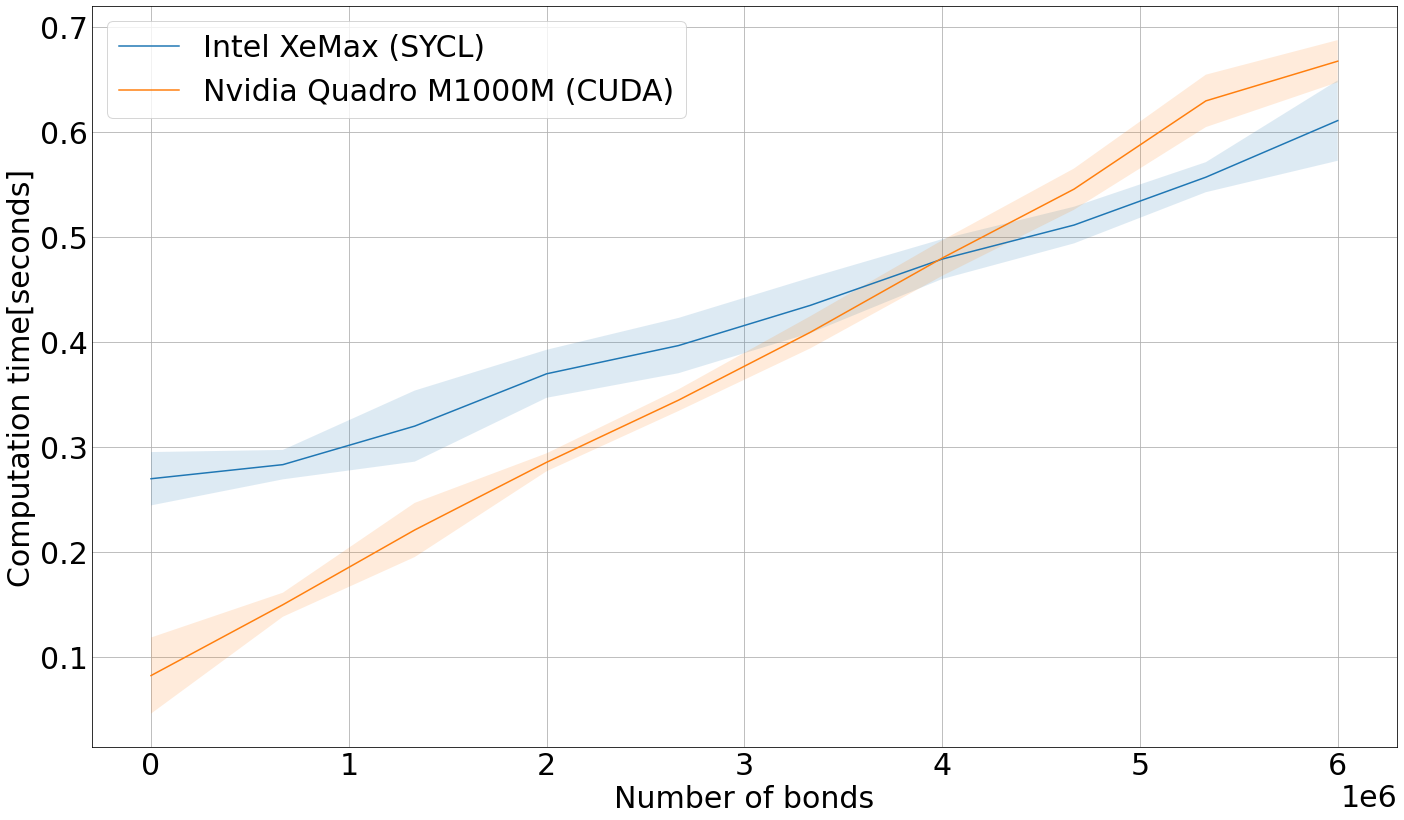
\includegraphics[width=0.75\textwidth]{openmm2.png}
	\label{fig:openmm}
\end{figure}

\subsubsection{Further Work for Porting OpenMM}\label{sec:openmm_furtherwork}

As has already been mentioned above there are two major parts of an OpenMM port to SYCL that have not addressed in this work these are 1) porting of all force kernels and 2) porting of dynamic code generation methods.
Before continuing to port more force kernels it is the opinion of the authors that porting of the dynamic code generation should be the next priority. The authors are aware of other codes which use run time compilation with SYCL (https://github.com/ginkgo-project/ginkgo) and so although porting OpenMM to SYCL would take significant effort to perform manually we are not aware of any reasons why it would not be possible.


\subsubsection{Effort Required for Porting OpenMM}\label{sec:openmm_effort}

The authors of this section were novices in CUDA programming and new to SYCL programming as such the results here should represent the effort required for a port to be achieved by user new to GPU programming.
Porting of the bonded kernel can be considered as three tasks 1) learning sufficient CUDA to understand the problem and 2) converting the extracted code using the Intel compatibility tool.
The authors estimate that task 1) was the most time consuming with a rough estimate of 1--2 PM (person-month) but task 2), once the CUDA kernel was in hand and well understood, was much faster and took on the order of 0.25 PM.
From the perspective of a GPU programming novice we comment that the porting of a single kernel from CUDA to SYCL was very straight forward provided the CUDA API in the code being ported is supported.
We have found in this part of the work sections of the CUDA API that are not supported, namely nvrtc.
Without the support of Intel compatibility tool it is the opinion of this author that the complexity to port a code such as OpenMM is well beyond what is possible for a novice.

\end{document}

% chktex-file 13
% chktex-file 44
% chktex-file 24

\documentclass[../main]{subfiles}

\begin{document}

\subsection{HemeLB}\label{sec:hemelb}

Computational fluid dynamics represents a significant use case for high performance computing in many fields of engineering and science.
Of the many techniques available in this field, the lattice Boltzmann method (LBM) has gained traction in the community for its ability to be both simply deployed for parallel computation and its facility to handle complex geometric and moving boundary conditions.
The HemeLB code\footnote{\url{https://github.com/hemelb-codes}} uses the LBM to study 3D blood flow in human-scale vascular domains and has been optimised to handle the sparse geometries characteristic of these problems.
In previous work, the CPU version of the code has been shown to display strong scaling to over 300,000 cores on SuperMUC-NG (\textbf{citation}) whilst a GPU port of the code has displayed similar characteristics to over 18,000 NVIDIA V100 GPUs on Summit~\cite{zacharoudiou_development_2022}.

The current GPU ports of HemeLB have been developed using the CUDA framework.
Whilst this has been suitable for the current generations of HPC infrastructure, the imminent arrival of alternative accelerator hardware has necessitated the implementation of more platform-agnostic coding structures.
This effort porting to the OneAPI platform will be instructive as to the level of complexity of such a migration for a mature, detailed and highly performant application.

The OneAPI platform advocates the use of its DPCT conversion tool to convert the majority of an existing CUDA code to the DPC++ framework.
From a practical standpoint, it can be noted that the DevCloud environment that is offered for DPC++ development does not appear to natively contain the CUDA header files necessary for the conversion of an existing CUDA code with DPCT to take place.
As such, conversion needs to be done locally or on a cluster that contains both CUDA and OneAPI software.
Additionally, the majority of resources on the use of DPCT focus on simple, single file, examples of CUDA code.
In reality, porting a mature code will require the conversion and correction of several files to ensure a fully operational application is able to be compiled.
This is further complicated by features such as MPI communication between multiple GPUs.
For this current exercise, we have extracted a single HemeLB collision kernel to test the performance variation between a native CUDA implementation and that converted to DPC++.
The chosen kernel computes the single-relaxation time collision function used by the LBM to solve fluid flow within the simulation domain.
This is used to update the vast majority of sites at each time step and represents the bulk of computation within an iteration.

This kernel was extracted from the main HemeLB code and written into a single CUDA file with appropriate supporting structures and data to allow it to run on a single GPU.
This, highly simplified, script was converted to DPC++ with DPCT.
On our first attempt, the conversion yielded one error that needed to be corrected by hand.
Here it failed to convert a declaration of a constant memory array despite successfully converting several around the same location:

\begin{lstlisting}[language=C++,basicstyle=\small]
dpct::constant_memory<int, 1> _InvDirections_19(19); <--- Converted successfully
//__constant__ double _EQMWEIGHTS_19[19]; <--- Remained after DPCT conversion
dpct::constant_memory<double, 1> _EQMWEIGHTS_19(19); <--- Manually added
dpct::constant_memory<int, 1> _CX_19(19); <--- Converted successfully
\end{lstlisting}

For a updated version of the script, this error no longer occurred.

\subsubsection{Performance Analysis --- Profiling}\label{sec:hemelb_performance}
Following the conversion, we compared the performance of the native CUDA code and the converted code on the NVIDIA A100 GPUs available on the CSD3 cluster.
We also compared this to the Intel GPUs available on the Intel DevCloud environment.
This hardware however should not be regarded as comparable to the A100 cards and these results demonstrate the capacity for cross-platform deployment.
For this test we ran the kernel for the equivalent of 5000 iterations of a 100,000 site domain.
This was repeated 10 times to obtain a fair estimate of the runtime.

\begin{center}
	\begin{tabular}{||c c c||}
		\hline
		Hardware    & Code  & Average Runtime [s]     \\ [0.5ex]
		\hline\hline
		NVIDIA A100 & CUDA  & 0.398578 +/- 0.00020542 \\
		\hline
		NVIDIA A100 & DPC++ & 0.436205 +/- 0.00793029 \\
		\hline
		Intel P630  & DPC++ & 15.4501 +/- 0.0939887   \\ [1ex]
		\hline
	\end{tabular}
\end{center}

For this initial test case, it can be seen that on the common hardware tested here the conversion to the DPC++ framework and clang compiler has resulted in a 10\% drop in performance compared to the native CUDA code and NVIDIA compiler.

\begin{figure}[htp]
	\centering
	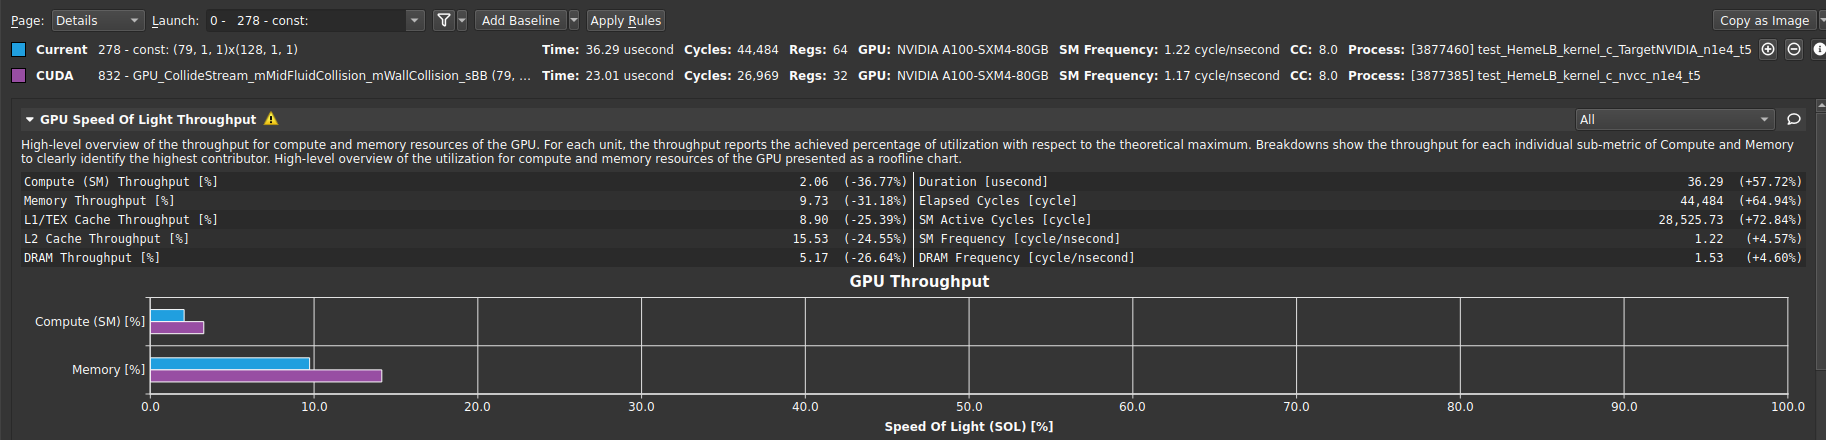
\includegraphics[clip,width=\textwidth]{Nsight_Compute_CUDA_vs_DPC++_A100_GPU.png}
	\caption{Profiling the CUDA and ported DPC++ code using NVIDIA's Nsight Compute on A100 GPU.}
	\label{fig:ncu_CUDA_Vs_DPC++_A100GPU}
\end{figure}

Profiling both versions of the code (CUDA, DPC++) was carried out using NVIDIA's performance analysis tools, Nsight Compute (see fig.~\ref{fig:ncu_CUDA_Vs_DPC++_A100GPU}) and Nsight Systems (see fig.~\ref{fig:nsys_DPC++_A100GPU}).
Nsight Compute provides detailed performance metrics at the kernel level and enables comparison of both versions, although we are not certain about the reliability of the results reported for the DPC++ code.
Nsight Compute reports a 37\% reduction of the compute throughput and a 58\% increase of the kernel's execution time compared to CUDA, while a $\sim10\%$ reduction in overall computational time was reported using either CPU timers (chrono library) or CUDA-specific timers (CUDA event API).
One issue we came across was that the profiler did not return the kernel's name for the DPC++ code.
This information was deducted from the launch statistics (gridsize and blocksize) that matched the corresponding values from profiling the native CUDA code.
The DPC++ ported function (CUDA lernel) is labelled as `const:', instead of the proper kernel's name.


Similar issues are observed with Nsight Systems.
Furthermore, the memory transactions to/from the GPU global memory are reported as memory copies to/from the Host.


\begin{figure}[htp]
	\centering
	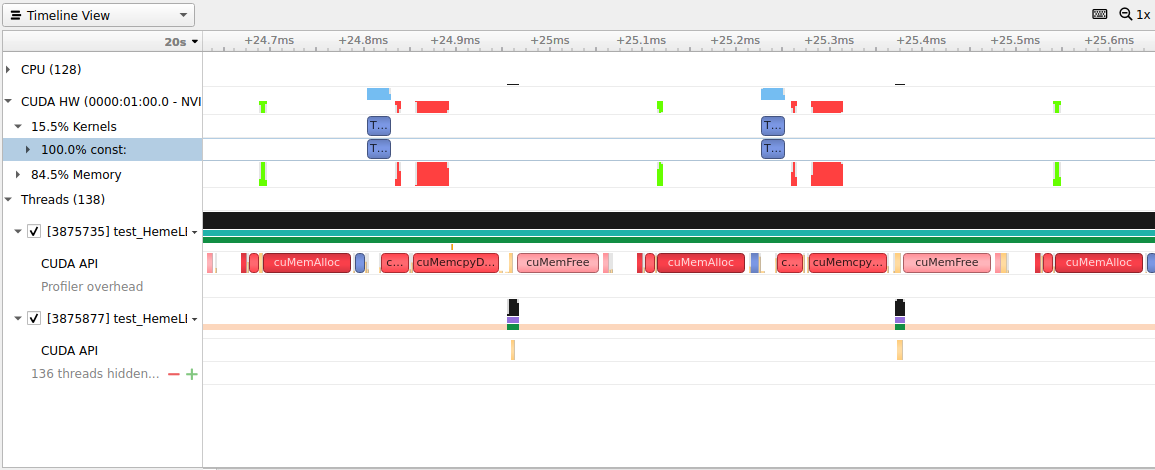
\includegraphics[clip,width=\textwidth]{profile_nsys_DPC++_A100_2steps.png}
	\caption{Profiling the ported DPC++ code using NVIDIA's Nsight Systems on A100 GPU.}
	\label{fig:nsys_DPC++_A100GPU}
\end{figure}

In this porting exercise, we have only examined HemeLB's main fluid collision kernel.
With this proof-of-concept completed, the next step would be to work through the full version of the HemeLB code to fully port it to the DPC++ format.
Being a mature code, conducting such a project port will more strongly test the capabilities to effectively port MPI-parallelised CUDA code to the OneAPI framework.


\subsubsection{Porting the full HemeLB\_GPU code}
We further tried porting the full HemeLB\_GPU CUDA code to the OneAPI framework on CSD3. This is a more complex situation, as it involves migrating multiple files to DPC++ and relies on CMake to build and compile the project.    

HemeLB relies on a few dependencies (metis/parmetis, boost, ctemplate, tinyxml), which need to be installed prior to compiling the source code.  
Hence, one issue that needs to be resolved first is having the right modules for building/compiling dependencies and native source CUDA code, before repeating the same procedure for the ported DPC++ code.

The source files that need to be ported to DPC++ are the following: 
\begin{verbatim}
    src
    |- cuda kernels def decl
    ||- GPU Collide Stream Iolets.cu
    ||- GPU Collide Stream wall sBB Iolets.cu
    ||- cuda params.cu
    |
    |- lb
    ||- lb.hpp
    |
    |- net
    ||- BaseNet.cc
    |
    |- Geometry
    ||- LatticeData.cc
    |
    |- main.cu
    |
    |- Simulation Master.cu
\end{verbatim}

In principle, there are two approaches for migrating CUDA codes to DPC++. 
The first one involves a file-to-file manual migration, which is a good choice for migrating a few files.
For HemeLB, however, this is not the case. Hence, we follow an alternative approach, which relies on cmake and passing the compilation database (JSON file) to dpct for migrating the full project to DPC++.    
%For projects using CMake commands it is useful to create a JSON file. This will contain the build options of the input project's files, i.e. include path and macros definitions. 
The compilation database (compile\_commands.json file), containing the commands required to build the project, is generated by running 
\begin{verbatim}
    intercept-build make.
\end{verbatim}
%This creates the compile\_commands.json file. %(compilation database containing the commands required to build the project). 
%Next running dpct with the compilation database generates the full ported DPC++ code with a list of warnings that need to be addressed. 

The procedure for porting the full HemeLB code is therefore the following: 
\begin{enumerate}
    \item Create build directory, e.g. ``src/build"
    \item Within "src/build" run ``cmake ..''
    \item Run ``intercept-build make''. This generates the compilation database (compile\_commands.json) 
    \item Navigate one level up (src/). 
    \item Run 
    \begin{verbatim}
    dpct -p build/compile_commands.json --in-root=. \
        --out-root=../src_dpct_output --keep-original-code \
        --process-all
    \end{verbatim}
    \item Manually verify and edit the migrated code (in src\_dpct\_output/).
\end{enumerate}

During the migration stage the majority of the warnings received involved CUDA error checking functionalities added in HemeLB\_GPU. 
All CUDA runtime API calls return an error code (cudaError\_t is an enum type), while DPC++ uses exceptions to handle errors. Hence, the dpct tool added messages in the comments to indicate additional manual edits are likely necessary.
For example, warnings were issued for the following in the CUDA code:  
\begin{verbatim}
    cudaError_t error = cudaGetLastError();
    cudaError_t cudaStatus;
    cudaStatus = cudaMemcpy(dens_GPU, &(((distribn_t*)GPUDataAddr_dbl_MacroVars)[0]), MemSz, cudaMemcpyDeviceToHost);
    cudaStatus = cudaMalloc((void**)&GPUDataAddr_dbl_MacroVars, TotalMem_dbl_MacroVars);
\end{verbatim}

Warnings were also raised concerning the workgroup size passed to the SYCL ported kernel. For example:
\begin{verbatim}
    warning: DPCT1049:249: The workgroup size passed to the SYCL kernel 
    may exceed the limit. To get the device limit, 
    query info::device::max_work_group_size. 
    Adjust the workgroup size if needed.
\end{verbatim}

Finally, warnings were also issued for parameters declared in the CUDA code as ``extern"
\begin{verbatim}
    warning: DPCT1057:0: Variable _Iolets_Inlet_Edge was used in host code and 
    device code. The Intel(R) DPC++ Compatibility Tool updated _Iolets_Inlet_Edge 
    type to be used in SYCL device code and generated 
    new _Iolets_Inlet_Edge_host_ct1 to be used in host code. You need to update 
    the host code manually to use the new _Iolets_Inlet_Edge_host_ct1.
\end{verbatim}

\subsubsection{Compiling}
One problem detected is that the CMakeLists.txt file hasn't been adjusted accordingly after running the dpct compatibility tool. The source files that were modified (extension changed to *.dp.cpp) were not updated. In our case this involves the following files:
\begin{verbatim}
./main.dp.cpp
./SimulationMaster.dp.cpp
./geometry/GeometryReader.cc.dp.cpp
./geometry/decomposition/BasicDecomposition.cc.dp.cpp
./colloids/Particle.cc.dp.cpp
./net/BaseNet.cc.dp.cpp
./cuda_kernels_def_decl/GPU_Collide_Stream_Iolets.dp.cpp
./cuda_kernels_def_decl/cuda_params.dp.cpp
./cuda_kernels_def_decl/GPU_Collide_Stream_wall_sBB_Iolets.dp.cpp
./cuda_kernels_def_decl/initialise_GPU.dp.cpp
./extraction/SurfacePointSelector.cc.dp.cpp
./lb/kernels/rheologyModels/CarreauYasudaRheologyModel.cc.dp.cpp
./lb/iolets/InOutLetWomersleyVelocity.cc.dp.cpp
./lb/iolets/InOutLetCosine.cc.dp.cpp
\end{verbatim}

We had to manually modify the following files
\begin{verbatim}
    ./extraction/CMakeLists.txt
    ./geometry/CMakeLists.txt
    ./lb/CMakeLists.txt
    ./net/CMakeLists.txt
    ./colloids/CMakeLists.txt
\end{verbatim}
and modify the CMAKE\_CXX\_FLAGS in the CMakeLists.txt file
\begin{verbatim}
set(CMAKE_CXX_FLAGS "${CMAKE_CXX_FLAGS} -fsycl -fsycl-targets=nvptx64-nvidia-cuda")
\end{verbatim}

We had to adjust the C++ standard to at least 17
\begin{verbatim}
warning: DPCPP does not support C++ version earlier than C++17. 
Some features might not be available.
\end{verbatim}

Further compiling problems related to the pow function


\subsubsection{General Comments}
Generally, we must note that the warnings are clear and running the dpct compatibility tool for porting the full CUDA HemeLB\_GPU code is straightforward. This makes the porting process a task that even a developer with little to no experience in SYCL can still carry out.    



\subsubsection{Estimate of Development Effort}

\end{document}

% chktex-file 36
% chktex-file 44
% chktex-file 8

\documentclass[../main]{subfiles}

\begin{document}

\subsection{dGpoly3D}\label{sec:dgpoly3d}

Discontinuous Galerkin (dG) methods on meshes consisting of polytopic elements have received considerable attention in recent years.
By combining advantages from both finite element methods (FEMs) and finite volume methods (FVMs) they allow the simple treatment of complicated computational geometries, ease of adaptivity and stability for non-self-adjoint PDE problems.
It has also been shown that they are applicable on extremely general meshes, consisting of general polytopic elements with an arbitrary number of faces and different local elemental polynomial degrees.
A basic feature of these methods is the use of physical frame polynomial bases and this, together with the highly involved quadrature requirements over polytopic elements, pose new algorithmic challenges in the context of matrix assembly.
The implementation of arbitrary order quadrature rules over polytopic domains is non-trivial with the most general and widely used approach being the subdivision of polytopic elements into basic simplicial sub-elements; standard quadrature rules are then employed on each sub-element.
\texttt{dgpoly3d}~\cite{dong_gpu-accelerated_2021} is a CUDA implementation of the symmetric interior penalty dG method, for the linear system assembly step of second order advection-diffusion-reaction equations.

The code first subdivides each 3D polytopic element into simplicial sub-elements (tetrahedrons) and any co-hyperplanar 2D faces into simplicial sub-faces (triangles), it then precomputes the sparsity pattern of the stiffness and mass matrix and stores it in CSR format and finally populates the matrix with the quadrature values for each simplex of the simplicial subdivision.
Different kernels are called for each term of the bilinear form, since the workload of each term can be substantially different.
For example, the kernel that calculates the integral over the elements needs a 3D quadrature rule, compared to the kernel over the interior faces which needs a 2D quadrature rule and thus less integration points.
For this project we will port one of the kernels, the kernel over the elemental integrals.
This kernel spawns as many threads as there are tetrahedrons on the mesh and for each tetrahedron it computes the contribution of this simplex and writes it into the main block diagonal of the matrix using atomic operations.
Atomic operations are needed since threads with contiguous thread id's might belong in the same polyhedron and thus will try to update the same memory location simultaneously.

\subsubsection{Preparing the code}\label{sec:dgpoly3d_prep}
The code is a combination of Python scripts for the non computationally demanding parts along with native CUDA kernels for the matrix assembly process, called from within Python with the PyCUDA module.
The code was executed for different mesh sizes and with $p=2$ (the degree of the polynomial on every polyhedron) and input and output data to and from the kernel were captured and stored, both to be able to execute the kernel without having to do the initialization steps every time but also to be used in a unit test.

Since Intel's DPC++ Compatibility tool would not be able to port the CUDA API calls (written in PyCUDA), a minimal C++ code to drive the kernel was written.
This code reads the input and output data from disk, performs the memory transfers from and to the device, calls the kernel and finally the unit test.
The unit test checks if the matrix entries match within a tolerance with the original values and for this a C++ version of Python's float comparison \texttt{math.isclose()} function was written, that takes as parameters both a relative and an absolute tolerance and returns True if
\begin{verbatim}
abs(x - y) <= max(rel_tol * max(abs(x), abs(y)), abs_tol))
\end{verbatim}
otherwise it returns False.
For the following comparisons we've set the relative tolerance to $1\%$ and the absolute to $10^{-5}$.

\subsubsection{Porting the code}\label{sec:dgpoly3d_porting}
We ported the code using Intel's DPC++ Compatibility tool (\texttt{dpct}).
Porting completed without errors and the compatibility tool added inline comments to explain some of its decisions or even propose changes (for example in one place where we access with atomic operations an array residing in global memory, it proposed a change in case the array is in local memory instead).
We also automatically created a \texttt{Makefile} with the \texttt{--gen-build-script} flag.
However, compiling failed with the following error message:
\begin{verbatim}
  no known conversion from 'dpct::accessor<float,
  dpct::constant, 2>' 'float (*)[3]' for 1st argument
\end{verbatim}
The problem was found to be with the function call that evaluates the Legendre polynomials at a given point.
In the CUDA code, the coefficients of the Legendre polynomials are stored in the GPU's constant memory
\begin{verbatim}
  __constant__ float legendre[3][3];
\end{verbatim}
and are passed to the \texttt{eval1dLegendre0()} and \texttt{eval1dLegendre1()} function calls to evaluate the Legendre polynomial and its first derivative and the function declaration is
\begin{verbatim}
  __device__ float eval1dLegendre0(float legendre[][3], int n, float x);
\end{verbatim}
After porting the code, while the declaration of the constant memory was changed to
\begin{verbatim}
  dpct::constant_memory<float, 2> legendre(3, 3);
\end{verbatim}
and it was included in the kernel call as
\begin{verbatim}
  dpct::accessor<float, dpct::constant, 2> legendre
\end{verbatim}
the type was not changed in the \texttt{eval1dLegendre} function.
After changing the parameter type for the first argument in the function definition from \texttt{float legendre[][3]} to \texttt{dpct::accessor<float, dpct::constant, 2> legendre} the ported code compiled succesfully.

\subsubsection{Running the code}\label{sec:dgpoly3d_running}
To start with, the simplified native CUDA code was tested on a workstation with an Nvidia 2060 (Turing) and in an HPC GPU cluster with A100's (Ampere).
In the first case we used CUDA SDK 11.6 and on the GPU cluster we compiled with CUDA SDK 11.4.
We also compiled it with the optimization levels \texttt{-O0} up to \texttt{-O3} and with or without the \texttt{-use\_fast\_math} flag and in all cases the unit test passed with no errors.

Now, for the ported SYCL/DPC++ code multiple different platforms were used, both CPU based and GPU based.
The GPU was once again the Nvidia Ampere A100 and the CPU based systems were one with dual Intel Icelake 8368Q and one with dual AMD EPYC 7763.
To target the Nvidia GPU we compiled with the LLVM CUDA backend compiler with \texttt{clang++ -fsycl -fsycl-targets=nvptx64-nvidia-cuda} and to target the CPU we compiled with both the DPC++ compiler (\texttt{dpcpp}) and with Intel's LLVM with \texttt{clang++ -fsycl} (which by default selects the generic spir64 target).
The results of the unit test can be found on Table~\ref{tab:correctness}.

\begin{table}[!htbp]
	\begin{tabular}{@{}c c c c c@{}}
		\toprule
		    & \multicolumn{2}{c}{\textbf{dpcpp}} & \multicolumn{2}{c}{\textbf{clang++}}                               \\
		\cmidrule(lr){2-3}\cmidrule(lr){4-5}
		    & {Icelake 8368Q}                    & EPYC 7763                            & Icelake 8368Q & Ampere A100 \\
		\midrule
		-O0 & \qty{0.54507}{\percent} wrong      & \qty{0.54507}{\percent} wrong        & ---           & correct     \\
		-O1 & \qty{1.20335}{\percent} wrong      & \qty{1.20545}{\percent} wrong        & correct       & correct     \\
		-O2 & \qty{1.20335}{\percent} wrong      & \qty{1.20545}{\percent} wrong        & correct       & correct     \\
		-O3 & \qty{1.20335}{\percent} wrong      & \qty{1.20545}{\percent} wrong        & correct       & correct     \\
		\bottomrule
	\end{tabular}
	\caption{\label{tab:correctness}}
\end{table}

Further investigation suggests that this behaviour is due to different default semantics for floating point calculations between the two different compilers.
According to Table~\ref{tab:semantics} the default model in \texttt{dpcpp} is \texttt{fast} while in \texttt{clang++} is \texttt{precise}.

\begin{table}[!htbp]
	\begin{tabular}{@{}lll@{}}
		\toprule
		\multirow{4}{*}{\texttt{dpcpp -O1}}          & ---                          & \qty{1.20335}{\percent} wrong \\
		                                             & \texttt{-fp-model=fast   }   & \qty{1.20335}{\percent} wrong \\
		                                             & \texttt{-fp-model=strict }   & \qty{0.54507}{\percent} wrong \\
		                                             & \texttt{-fp-model=precise}   & correct                       \\
		\midrule
		\multirow{4}{*}{\texttt{clang++ -fsycl -O1}} & ---                          & correct                       \\
		                                             & \texttt{-ffp-model=fast    } & \qty{1.20335}{\percent} wrong \\
		                                             & \texttt{-ffp-model=strict }  & \qty{0.54507}{\percent} wrong \\
		                                             & \texttt{-ffp-model=precise}  & correct                       \\ \bottomrule
	\end{tabular}
	\caption{\label{tab:semantics}}
\end{table}

\end{document}


\subsection{AREPO}\label{sec:arepo}

Arepo is a massively parallel astrophysics code for the simulation of gravitational N-body systems and magnetohydrodynamics, both on Newtonian as well as cosmological backgrounds. There are a number of versions in the community, originating from a common closed-source code base. A version with reduced functionality was made publicly available under GPLv3\cite{weinberger_arepo_2020, springel_arepo_nodate}. Different research groups use code bases derived from the closed source version, including the Sijaki group at the University of Cambridge. This code \cite{sijaki_arepo_nodate}, which was part of the DiRAC3 procurement, acceptance testing and technical commissioning, forms the basis of porting efforts to be undertaken within the course of this project.

In Arepo, the computational domain is discretized using a fully adaptive, dynamic unstructured Voronoi mesh, which is moving with the fluid in a quasi-Lagrangian way and that is paired with a finite volume approach for the hydrodynamics.
Arepo is written in C, parallelized with MPI and some of the code bases, including the one used in this project, have additionally OpenMP shared memory parallelization. To the best of our knowledge, there is currently no version of this code that can target accelerators with any of the computational kernels in the main time loop.
As a C application that includes already OpenMP parallelization, we intend to follow Intel's recommendation to use OpenMP 5 offloading to target GPUs.

%In order to run simulations efficiently on the next generation of supercomputers there are a few key aspects that need to be taken into account. Some of those steps are already well known in the HPC community for years, i.e. well balanced computational load or the avoiding collective communication as much as possible. Apart from that it will be increasingly important to make use of hybrid architectures, i.e. accelerators.
In contrast to codes described above, where suitable kernels for GPU execution have already been identified in prior porting efforts, this selection process has to be done as an additional first step for this purely CPU-based code. Therefore, extensive profiling of the code base has been undertaken using one of the test cases that are also used to verify code correctness to analyze the potential of porting parts of Arepo to GPUs. Hence, a first analysis was carried out using Intel VTune profiler and Intel Trace Analyzer, producing two key insights:

The first insight was that a significant share of the overall run time is spent waiting in a synchronisation step that uses global MPI communication. The purpose of this step is to detect the need for program interruption to trigger saving the current state in a snapshot file and termination of the program. Since there is no data dependence on this communication step, it is possible to reverse the logic of this routine, replace the respective MPI calls with their non-blocking counterparts and trigger the snapshot writing after the next time step. This enables perfect overlap of computation and communication at the expense of a one time step lag in the snapshot writing. Even on this small single-node test case this already reduces the run time of the main time loop by 2\%, promising even larger savings in production runs that use significantly more nodes.

\begin{figure}[htp]
	\centering
	\subfloat{ 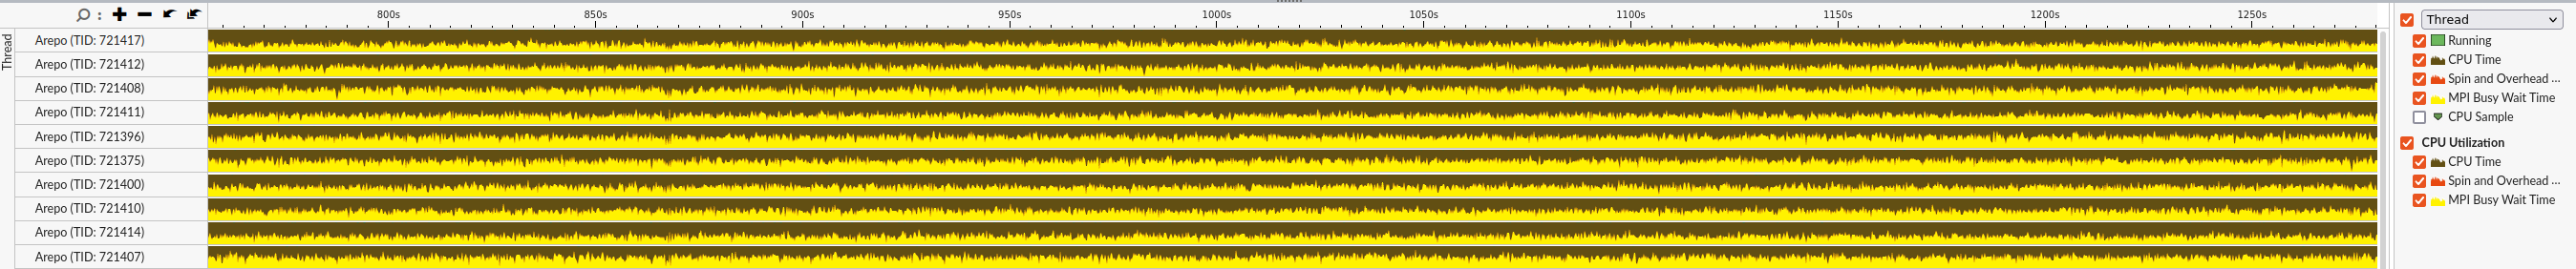
\includegraphics[clip,width=\textwidth]{arepo_blocking.png}}
	\subfloat{ 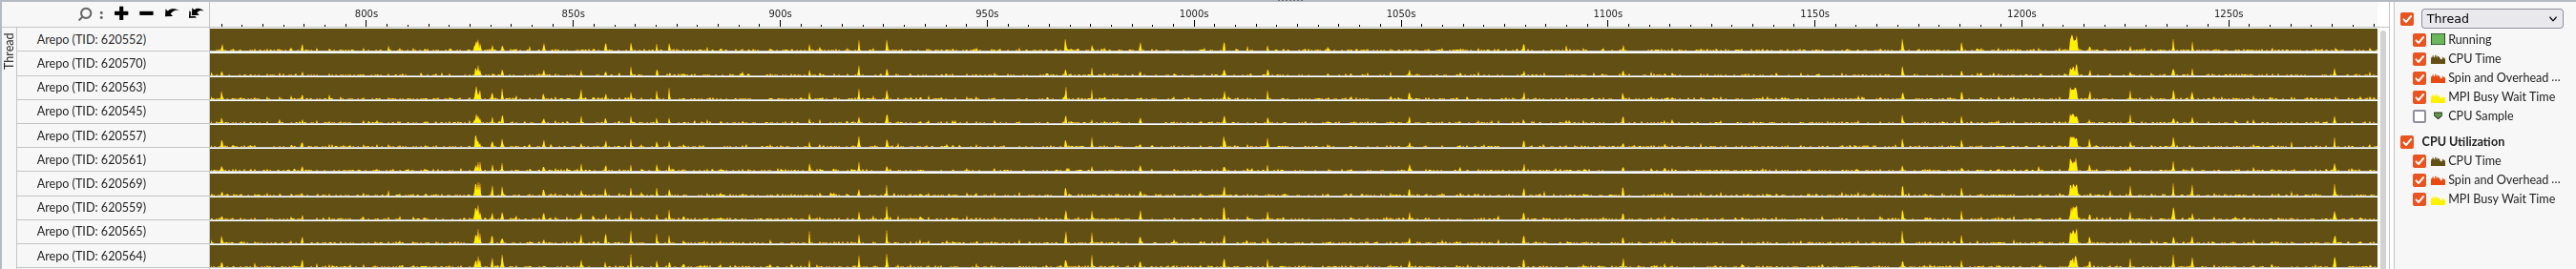
\includegraphics[clip,width=\textwidth]{arepo_nonblocking.png}}
	\caption{Significant reduction of MPI Busy Wait Time (yellow) in the lower VTune Profiler graphic compared to the top version where blocking communication was used. Shown for a random selection of ranks}
	\label{fig:arepo_mpicom}
\end{figure}

Second profiling outcome and original motivation for this analysis was to understand the distribution of run time across the different parts of a time step and subsequently to identify suitable candidates for GPU porting. The two most time-consuming parts proved to be the evaluation of gravitational forces, which is carried out in two half steps at the beginning and end of a time step, and the creation of the Voronoi mesh in-between.

The next step in the analysis was to use Intel's Offload Advisor to see if these contain any kernels that would readily benefit from GPU offloading. However, with the current structure of the underlying algorithm the Offload Advisor judged every routine to suffer from too much overhead when ported to GPU. Only relatively short loops within sub steps of the mesh creation routines were classified as offload candidates that could potentially see any speed-up.

Overall, this suggests that for a successful GPU port of Arepo it may not be sufficient to port few individual kernels to achieve performance gains but requires a better understanding of the numerical method and possibly adaptation of the algorithm to better map to the target hardware. For that, we are in active discussions with the developers at the University of Cambridge and take into account prior experience and publications in the scientific domain.

%\begin{itemize}
%    \item reference to paper to port
%    \item https://arxiv.org/abs/1610.07279
%    \item https://arxiv.org/abs/0907.3390
%    \item https://arxiv.org/abs/1909.07439
%\end{itemize}
